\section{Lecture 46.00: Post Stratification}
Until now what you had some strata, performed SRS on each stratum, then
combined them, and looked at the population value $ \mu $. See~\Cref{fig:strata}.
\begin{figure}[!htbp]
    \centering
    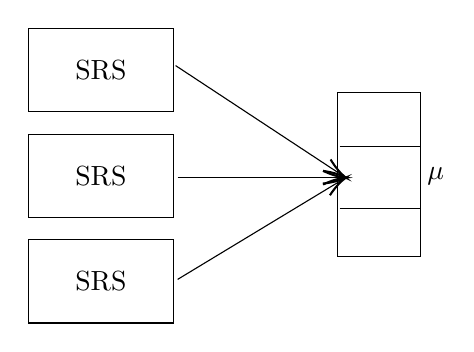
\begin{tikzpicture}[x=0.75pt,y=0.75pt,yscale=-1,xscale=1]
        %uncomment if require: \path (0,162); %set diagram left start at 0, and has height of 162

        %Shape: Rectangle [id:dp6861764355714591] 
        \draw   (12,9) -- (82,9) -- (82,49) -- (12,49) -- cycle ;
        %Shape: Rectangle [id:dp7925417207393711] 
        \draw   (12,60) -- (82,60) -- (82,100) -- (12,100) -- cycle ;
        %Shape: Rectangle [id:dp9116080179254983] 
        \draw   (12,111) -- (82,111) -- (82,151) -- (12,151) -- cycle ;
        %Straight Lines [id:da42452853568114324] 
        \draw    (83,27) -- (163.33,79.9) ;
        \draw [shift={(165,81)}, rotate = 213.37] [color={rgb, 255:red, 0; green, 0; blue, 0 }  ][line width=0.75]    (10.93,-3.29) .. controls (6.95,-1.4) and (3.31,-0.3) .. (0,0) .. controls (3.31,0.3) and (6.95,1.4) .. (10.93,3.29)   ;
        %Straight Lines [id:da2851258632117559] 
        \draw    (84,81) -- (163,81) ;
        \draw [shift={(165,81)}, rotate = 180] [color={rgb, 255:red, 0; green, 0; blue, 0 }  ][line width=0.75]    (10.93,-3.29) .. controls (6.95,-1.4) and (3.31,-0.3) .. (0,0) .. controls (3.31,0.3) and (6.95,1.4) .. (10.93,3.29)   ;
        %Straight Lines [id:da06580588611951421] 
        \draw    (84,130) -- (163.29,82.04) ;
        \draw [shift={(165,81)}, rotate = 508.83] [color={rgb, 255:red, 0; green, 0; blue, 0 }  ][line width=0.75]    (10.93,-3.29) .. controls (6.95,-1.4) and (3.31,-0.3) .. (0,0) .. controls (3.31,0.3) and (6.95,1.4) .. (10.93,3.29)   ;
        %Shape: Rectangle [id:dp33582592326822736] 
        \draw   (161,40) -- (201,40) -- (201,119) -- (161,119) -- cycle ;
        %Straight Lines [id:da11175824112302257] 
        \draw    (162,66) -- (201,66) ;
        %Straight Lines [id:da37350978775751853] 
        \draw    (162,96) -- (201,96) ;

        % Text Node
        \draw (203,80.2) node [anchor=west] [inner sep=0.75pt]    {$\mu $};
        % Text Node
        \draw (47,29) node   [align=left] {SRS};
        % Text Node
        \draw (47,80) node   [align=left] {SRS};
        % Text Node
        \draw (47,131) node   [align=left] {SRS};
    \end{tikzpicture}
    \caption{Regular Stratification}\label{fig:strata}
\end{figure}
In post stratification, the idea is that you have done an SRS
of some large population, and then decided afterwards that you wanted to stratify.
At this point, you then break it into three.
Notice that the SRS is done at the \emph{start} as opposed to at the \emph{end}.
See~\Cref{fig:post_strata}.
\begin{figure}[H]
    \centering
    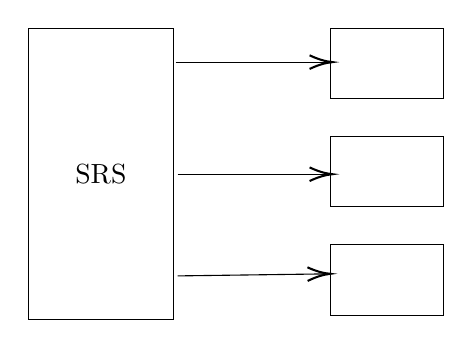
\begin{tikzpicture}[x=0.75pt,y=0.75pt,yscale=-1,xscale=1]
        %Shape: Rectangle [id:dp9116080179254983] 
        \draw   (12,11) -- (82,11) -- (82,151) -- (12,151) -- cycle ;
        %Straight Lines [id:da42452853568114324] 
        \draw    (83,27) -- (156.5,27) ;
        \draw [shift={(158.5,27)}, rotate = 180] [color={rgb, 255:red, 0; green, 0; blue, 0 }  ][line width=0.75]    (10.93,-3.29) .. controls (6.95,-1.4) and (3.31,-0.3) .. (0,0) .. controls (3.31,0.3) and (6.95,1.4) .. (10.93,3.29)   ;
        %Straight Lines [id:da2851258632117559] 
        \draw    (84,81) -- (156.5,81) ;
        \draw [shift={(158.5,81)}, rotate = 180] [color={rgb, 255:red, 0; green, 0; blue, 0 }  ][line width=0.75]    (10.93,-3.29) .. controls (6.95,-1.4) and (3.31,-0.3) .. (0,0) .. controls (3.31,0.3) and (6.95,1.4) .. (10.93,3.29)   ;
        %Straight Lines [id:da06580588611951421] 
        \draw    (84,130) -- (155.5,129.03) ;
        \draw [shift={(157.5,129)}, rotate = 539.22] [color={rgb, 255:red, 0; green, 0; blue, 0 }  ][line width=0.75]    (10.93,-3.29) .. controls (6.95,-1.4) and (3.31,-0.3) .. (0,0) .. controls (3.31,0.3) and (6.95,1.4) .. (10.93,3.29)   ;
        %Shape: Rectangle [id:dp39278086756839947] 
        \draw   (157.5,115) -- (212,115) -- (212,149) -- (157.5,149) -- cycle ;
        %Shape: Rectangle [id:dp5029651538179899] 
        \draw   (157.5,62.67) -- (212,62.67) -- (212,96.67) -- (157.5,96.67) -- cycle ;
        %Shape: Rectangle [id:dp3267534023424148] 
        \draw   (157.5,10.67) -- (212,10.67) -- (212,44.67) -- (157.5,44.67) -- cycle ;
        % Text Node
        \draw (47,81) node   [align=left] {SRS};
    \end{tikzpicture}
    \caption{Post Stratification}\label{fig:post_strata}
\end{figure}
Mathematically, your sample sizes end up being random, which has an influence on how
we calculate things. Although, it doesn't actually have an influence
on the actual mathematics at the end of the day, so the resultants are the same.
For example, the post stratification estimate is very similar to that of stratified:
\[ \hat{\mu}_{\text{post}}=w_1\mu_1+\cdots+w_H\mu_H \]
The estimated variance for post stratification is:
\[ \widehat{\Var*{\tilde{\mu}_{\text{post}}}}=\sum_{i=1}^{H} w_i^2\biggl(1-\frac{n_i}{N_i}\biggr)\frac{\hat{\sigma}_i^2}{n_i}  \]
A confidence interval for $ \mu_{\text{post}} $ is given by:
\[ \hat{\mu}_{\text{post}}\pm c\sqrt{\widehat{\Var*{\tilde{\mu}_{\text{post}}}}}\quad\text{where $ c \sim \N{0,1} $} \]
